\usetikzlibrary{arrows.meta,positioning,shapes.geometric}

\chapter{Prototype}%
\label{ch:prototype}

Dit project werd initieel opgezet als een proof-of-concept om de haalbaarheid van een automatische prijsvergelijker te evalueren. Tijdens de implementatie evolueerde het prototype echter naar een robuust en modulair systeem, met een duidelijke scheiding van verantwoordelijkheden en ondersteuning voor schaalbare dataverwerking. De webscrapingapplicatie is ontworpen met het oog op bruikbaarheid voor een breed publiek — met name studenten — dat niet beschikt over uitgebreide kennis van programmeren of softwareontwikkeling. De gebruiker heeft enkel een internetverbinding nodig en hoeft geen technische configuraties uit te voeren om het systeem te gebruiken.

Hoewel het project in zijn huidige vorm niet als volledig uitgerolde productieapplicatie kan worden beschouwd, biedt het wel een realistisch en werkbaar kader om inzicht te krijgen in moderne webscrapingarchitecturen. Het gebruik van Docker en een testomgeving maakt het mogelijk om het systeem lokaal te runnen en te experimenteren met de verschillende componenten, wat bijdraagt aan het educatieve karakter van het prototype.

Deze doelstelling impliceert dat de technische complexiteit van web scraping volledig wordt afgeschermd van de eindgebruiker. Interacties met het systeem verlopen via een eenvoudige en intuïtieve gebruikersinterface, terwijl alle onderliggende processen — zoals het ophalen van webpagina’s, het verwerken en normaliseren van data, het omgaan met anti-scrapingmechanismen en de opslag van gegevens — volledig achter de schermen worden afgehandeld.


Het prototype ondersteunt:
\begin{itemize}
    \item gebruikersgestuurde productzoekopdrachten
    \item automatische prijsvergelijking over meerdere supermarkten
    \item een slimme winkelmandfunctionaliteit
    \item achtergrondverversing van prijsdata
    \item fouttolerante scraping van heterogene databronnen
\end{itemize}

Het prototype fungeert hiermee als een abstraherende laag tussen de gebruiker en de onderliggende scrapingsinfrastructuur. Hoewel het systeem niet perfect is en nog verschillende beperkingen kent, slaagt het er wel in om de kernideeën en doelstellingen van een automatische prijsvergelijker duidelijk te demonstreren. Het project toont aan hoe een dergelijke toepassing kan worden opgebouwd, welke technische uitdagingen daarbij komen kijken en hoe deze op een gestructureerde manier kunnen worden aangepakt.

\section{Keuze van programmeertaal en frameworks}

De keuze van programmeertaal en bijhorende frameworks vormt een essentiële ontwerpbeslissing binnen dit prototype. Literatuur toont aan dat verschillende programmeertalen geschikt zijn voor web scraping, waaronder Python, JavaScript en C\#. Op basis van vergelijkende studies en best practices \autocite{BestPractice2025, PvsJS} is Python gekozen als primaire programmeertaal voor het prototype.

Deze keuze voor Python kan gemotiveerd worden door meerdere factoren. Ten eerste beschikt Python over een uitgebreid ecosysteem van bibliotheken die specifiek ontworpen zijn voor interactie met de inhoud van websites, zoals \textit{Requests}, \textit{BeautifulSoup}, \textit{Scrapy} en \textit{Playwright}. Hierdoor kan snel en efficiënt worden ingespeeld op uiteenlopende scrapingsuitdagingen, variërend van eenvoudige HTML-pagina’s tot complexe, dynamisch gegenereerde webinhoud. 
Ten tweede is Python relatief eenvoudig aan te leren, wat het bijzonder geschikt maakt voor beginnende ontwikkelaars en studenten. De leesbaarheid van de syntaxis en de grote hoeveelheid beschikbare documentatie en voorbeelden verlagen de instapdrempel aanzienlijk. Dit sluit aan bij de doelstelling van dit prototype, namelijk het ontwikkelen van een systeem dat toegankelijk is voor gebruikers zonder diepgaande programmeerkennis.
Tot slot biedt Python voldoende mogelijkheden voor toekomstige uitbreidingen, zoals grootschalige dataverwerking, data-analyse en integratie van machine learning technieken. Hierdoor is Python niet alleen geschikt voor het huidige prototype, maar ook toekomstbestendig.

Binnen het Python-ecosysteem bestaan meerdere bibliotheken voor web scraping. Na een vergelijking werd gekozen voor \textit{Scrapy} als centraal scrapingsframework. Deze keuze kan onderbouwd worden door het werk van \autocite{Eyzenakh2021}, waarin verschillende scrapingsoplossingen zijn vergeleken op vlak van performantie, schaalbaarheid en architecturale opbouw. Scrapy onderscheidt zich van eenvoudigere oplossingen zoals \textit{Requests} en \textit{BeautifulSoup} door zijn asynchrone en event-gedreven architectuur. Dit maakt het mogelijk om meerdere webpagina’s gelijktijdig te verwerken, wat resulteert in betere prestaties en efficiënter gebruik van systeembronnen. 
Daarnaast voorziet Scrapy ingebouwde ondersteuning voor request scheduling, foutafhandeling, throttling en uitbreidbare pipelines voor dataverwerking. Een bijkomend voordeel van Scrapy is de duidelijke scheiding tussen verschillende verantwoordelijkheden, zoals het ophalen van data, het parsen van responses en het verwerken van resultaten. Deze modulaire opbouw sluit nauw aan bij de architecturale principes die in de literatuur worden beschreven en verhoogt de onderhoudbaarheid van het systeem.

Hoewel Scrapy krachtig is voor het verwerken van statische HTML-pagina’s, volstaat het niet in alle situaties. Steeds meer websites maken gebruik van JavaScript om inhoud dynamisch te genereren. Om deze pagina’s correct te kunnen verwerken, werd \textit{Playwright} geïntegreerd in het scrapingsproces.
Playwright maakt het mogelijk om een echte browseromgeving te simuleren en JavaScript-code uit te voeren alvorens de HTML wordt geëxtraheerd. Hierdoor kunnen ook websites met complexe client-side logica succesvol gescrapet worden. De combinatie van Scrapy en Playwright zorgt voor een flexibele aanpak waarbij per website de meest geschikte scrapingstrategie kan worden toegepast. 

Om de verschillende lagen binnen het systeem van elkaar te ontkoppelen, werd gekozen voor Apache Kafka als verbindende component tussen de scrapingslaag en verdere verwerking van data. Kafka fungeert hierbij als een message broker die ruwe scrapingsresultaten doorstuurt naar volgende verwerkingsstappen.
De keuze voor Kafka is geïnspireerd door moderne, event-gedreven architecturen zoals beschreven in \autocite{Kafka2015}. Door gebruik te maken van een message broker wordt de afhankelijkheid tussen scraping en verwerking verminderd. Dit verhoogt de schaalbaarheid en fouttolerantie van het systeem en maakt het mogelijk om data opnieuw te verwerken zonder de scrapingsfase te herhalen.
Hoewel Kafka in dit prototype niet noodzakelijk op industriële schaal wordt ingezet, biedt het conceptueel een duidelijke meerwaarde en vormt het een solide basis voor toekomstige uitbreidingen.

Voor de backend van het prototype werd gekozen voor het Django-framework. Django sluit naadloos aan bij Python en biedt uitgebreide ondersteuning voor webapplicaties, databankintegratie en gebruikersinteractie.
Een belangrijk voordeel van Django is de eenvoudige koppeling met Python-gebaseerde scrapingscomponenten. Hierdoor kunnen scrapingsprocessen, dataverwerking en gebruikersinterface binnen één technologisch ecosysteem worden geïntegreerd. Daarnaast voorziet Django standaardfunctionaliteiten zoals ORM (Object-Relational Mapping), authenticatie en administratie, wat de ontwikkeltijd aanzienlijk verkort.

Om de reproduceerbaarheid en consistentie van het systeem op verschillende machines te garanderen, werd gebruikgemaakt van Docker. Docker maakt het mogelijk om de volledige applicatie, inclusief afhankelijkheden, configuraties en services, te verpakken in containers. Hierdoor kan het prototype zonder bijkomende installatieproblemen uitgevoerd worden op verschillende systemen, wat zowel de ontwikkeling als de evaluatie vereenvoudigt.

De combinatie van Python, Scrapy, Kafka, Django en Docker resulteert in een coherente en uitbreidbare architectuur waarin elke technologie een duidelijk afgebakende rol vervult.


\section{Klassieke web scraping pijplijn}

De structuur van web scraping systemen wordt in de literatuur vaak beschreven als een opeenvolging van afzonderlijke verwerkingsstappen. \autocite{Laender2002} beschrijft web data extractie als een pijplijn bestaande uit meerdere logisch gescheiden fasen: selectie van databronnen, extractie van ruwe data, transformatie en normalisatie, integratie en opslag.

Deze architecturale scheiding verhoogt de onderhoudbaarheid van het systeem en maakt hergebruik en schaalbaarheid mogelijk. Het prototype volgt deze pijplijnstructuur expliciet.
Op basis van de overleg met de co-promotor en de besproken state-of-the-art werd een modulaire architectuur voorgesteld. Deze architectuur is weergegeven in Figuur~\ref{fig:architectuur_overzicht}.

%\begin{figure}[h]
%    \centering
%    \includegraphics[width=0.9\textwidth]{scheme2.jpg}
%    \caption{Overzicht van de voorgestelde prototype-architectuur}
%    \label{fig:architectuur_overzicht}
%\end{figure}

\begin{figure}[H]
    \centering
    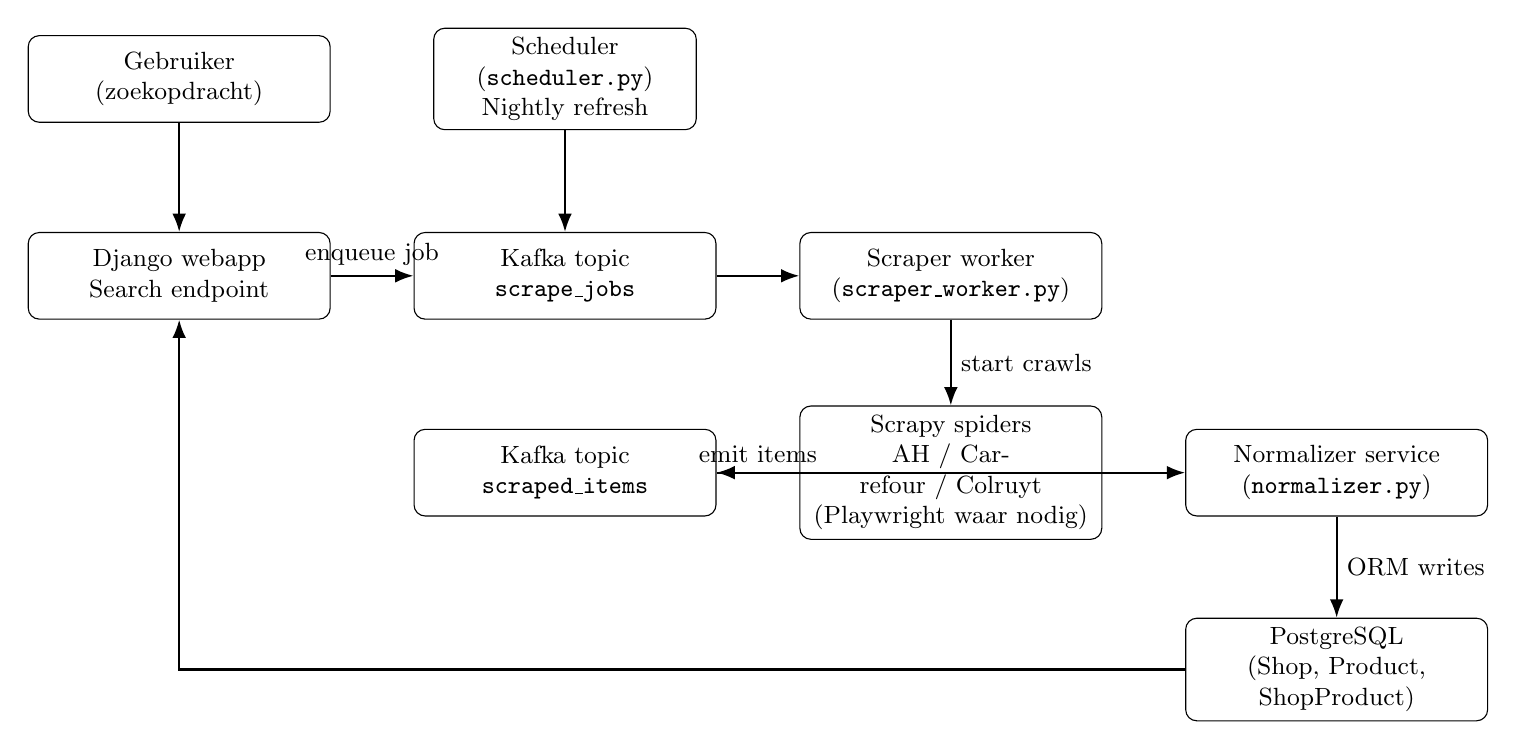
\begin{tikzpicture}[
        font=\small,
        box/.style={draw, rounded corners, align=center, text width=3.6cm, minimum height=1.1cm},
        smallbox/.style={draw, rounded corners, align=center, text width=3.1cm, minimum height=0.95cm},
        arrow/.style={-Latex, thick}
        ]
        % --- Grid coordinates (tune dx/dy if needed) ---
        \def\dx{4.9}   % column spacing
        \def\dy{2.5}   % row spacing
        
        % Left column
        \node[box] (user)   at (0,  \dy) {Gebruiker\\(zoekopdracht)};
        \node[box] (django) at (0, 0)    {Django webapp\\Search endpoint};
        
        % Middle-left column (Kafka)
        \node[box] (kafka_jobs)  at (\dx, 0)   {Kafka topic\\\texttt{scrape\_jobs}};
        \node[box] (kafka_items) at (\dx,-\dy) {Kafka topic\\\texttt{scraped\_items}};
        
        % Middle-right column (worker/spiders)
        \node[box] (worker)  at (2*\dx, 0)   {Scraper worker\\(\texttt{scraper\_worker.py})};
        \node[box] (spiders) at (2*\dx,-\dy) {Scrapy spiders\\AH / Carrefour / Colruyt\\(Playwright waar nodig)};
        
        % Right column (normalizer/db)
        \node[box] (normalizer) at (3*\dx,-\dy) {Normalizer service\\(\texttt{normalizer.py})};
        \node[box] (db)         at (3*\dx,-2*\dy) {PostgreSQL\\(Shop, Product, ShopProduct)};
        
        % Scheduler above kafka_jobs
        \node[smallbox] (scheduler) at (\dx, \dy) {Scheduler\\(\texttt{scheduler.py})\\Nightly refresh};
        
        % Arrows
        \draw[arrow] (user) -- (django);
        \draw[arrow] (django) -- node[above]{enqueue job} (kafka_jobs);
        \draw[arrow] (scheduler) -- (kafka_jobs);
        
        \draw[arrow] (kafka_jobs) -- (worker);
        \draw[arrow] (worker) -- node[right]{start crawls} (spiders);
        \draw[arrow] (spiders) -- node[above]{emit items} (kafka_items);
        
        \draw[arrow] (kafka_items) -- (normalizer);
        \draw[arrow] (normalizer) -- node[right]{ORM writes} (db);
        \draw[arrow] (db) -| (django);
        
    \end{tikzpicture}

    \caption{Event-driven scraping pipeline: Django publiceert scrape-jobs naar Kafka; de scraper worker voert spiders uit; resultaten worden genormaliseerd en opgeslagen in de database.}
    \label{fig:architectuur_overzicht}
\end{figure}




De architectuur van het project bestaat uit vijf hoofdlagen:
\begin{enumerate}
    \item Gebruikersinterface (Django)
    \item Scrapinglaag (Scrapy spiders)
    \item Ruwe datalaag (Kafka topics)
    \item Transformatielaag (Normalizer)
    \item Persistente databank (PostgreSQL)
\end{enumerate}

Figuur~\ref{fig:architectuur_overzicht2} toont een alternatief visueel overzicht van dezelfde lagen.

%\begin{figure}[h]
%\centering
%\includegraphics[width=0.9\textwidth]{scheme.jpg}
%\caption{Overzicht van de voorgestelde prototype-architectuur}
%\label{fig:architectuur_overzicht2}
%\end{figure}

\begin{figure}[H]
    \centering
    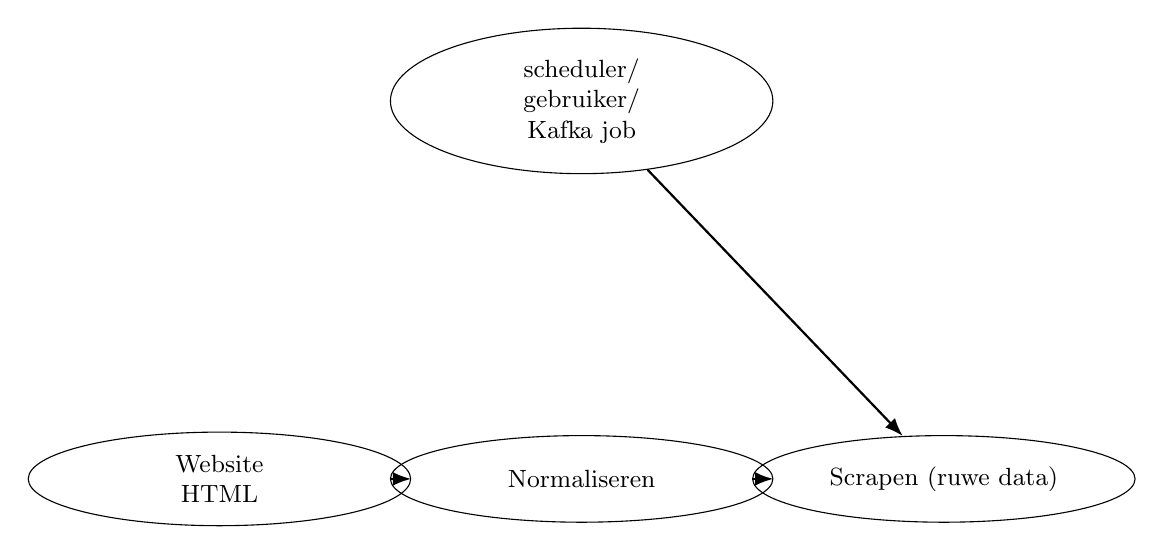
\begin{tikzpicture}[
        font=\small,
        box/.style={
            draw, rounded corners, align=center,
            text width=3.6cm, minimum height=1.1cm
        },
        oval/.style={
            draw, ellipse, align=center,
            text width=3.2cm, minimum height=1.1cm
        },
        arrow/.style={-Latex, thick}
        ]
        
        % --- Vertical spacing ---
        \def\dy{2.4}
        \def\dx{4.6}
        
        % --- Top: pacer / trigger ---
        \node[oval] (pacer) at (\dx, 2*\dy)
        {scheduler/\\gebruiker/\\Kafka job};
        
        % --- Bottom red area (scrape zone) ---
        \node[oval] (website) at (0, 0)
        {Website\\HTML};
        
        \node[oval] (raw) at (2*\dx, 0)
        {Scrapen (ruwe data)};
        
        % --- Transform ---
        \node[oval] (transform) at (\dx, 0)
        {Normaliseren};
        
        % --- Arrows ---
        \draw[arrow] (pacer) -- (raw);
        \draw[arrow] (raw) --  (transform);
        \draw[arrow] (transform) -- (website);

        
    \end{tikzpicture}
    \caption{Overzicht van de voorgestelde prototype-architectuur}
    \label{fig:architectuur_overzicht2}
\end{figure}


\section{Gebruikersinterface}

De gebruikersinterface vormt het enige directe contactpunt tussen de gebruiker en het systeem. Via deze interface kan de gebruiker producten opzoeken of een lijst van producten invoeren die vergeleken moeten worden over meerdere supermarkten. De gebruiker heeft geen zicht op, noch controle over, de onderliggende scraping- en verwerkingslogica; deze wordt volledig door het systeem afgehandeld.

De implementatie van de gebruikersinterface is gebaseerd op het Django-framework, dat fungeert als centrale coördinatielaag tussen de frontend, de databank en de asynchrone scraping-infrastructuur. 

\subsection{Rol van Django binnen het systeem}

Binnen dit project vervult Django een dubbele rol. Enerzijds verzorgt het framework de presentatie van gegevens via HTML-pagina’s en API-endpoints, anderzijds fungeert het als orkestrator die scraping-opdrachten initieert en de levenscyclus van zoekopdrachten bewaakt. Django is hierbij niet louter een presentatiecomponent, maar beheert actief de levenscyclus van zoekopdrachten. Django beslist op basis van bestaande data of een scraping-opdracht noodzakelijk is en fungeert daarbij als Kafka-producer. Indien data ontbreekt of verouderd is, publiceert Django een bericht naar het Kafka-topic \texttt{scrape\_jobs}. De verdere verwerking verloopt volledig asynchroon en zonder blokkering van de webserver.


\subsection{Data-architectuur en modellering}

Om frequente prijsupdates te ondersteunen en tegelijkertijd een duidelijke relatie tussen producten en winkels te behouden, werd de databank opgebouwd rond een genormaliseerd datamodel:

\begin{itemize}
    \item \texttt{Shop}: representeert een retailer (bv. Albert Heijn, Carrefour, Colruyt).
    \item \texttt{Product}: stelt een generiek product voor, los van een specifieke winkel (bv. “volle melk”).
    \item \texttt{ShopProduct}: vormt de verbindende entiteit tussen een \texttt{Shop} en een \texttt{Product}. Hier worden de effectieve prijsgegevens opgeslagen, waaronder \texttt{price\_amount}, \texttt{price\_per\_unit}, \texttt{source\_url} en \texttt{scraped\_at}.
\end{itemize}

Om dataconsistentie te garanderen werd een uniciteitsconstraint toegepast op de combinatie van product en winkel, zodat per winkel maximaal één actuele prijs per product wordt bijgehouden.

Daarnaast werden de modellen \texttt{SearchQueryRun} en \texttt{SearchResult} geïntroduceerd om zoekopdrachten en bijhorende resultaten historisch bij te houden. Deze modellen maken het mogelijk om herhaalde zoekopdrachten binnen een bepaalde tijdspanne te herkennen en onnodige scraping te vermijden.

\subsection{Zoekworkflow en asynchrone verwerking}

Wanneer een gebruiker een zoekopdracht uitvoert via de interface, wordt een vaste beslissingslogica toegepast:

\begin{enumerate}
    \item Eerst wordt de databank geraadpleegd om bestaande resultaten te vinden die overeenkomen met de zoekterm.
    \item Indien resultaten beschikbaar zijn, wordt gecontroleerd of de bijhorende \texttt{scraped\_at}-timestamp recenter is dan een vooraf gedefinieerde drempel (24 uur).
    \item Indien geen resultaten beschikbaar zijn, of indien de data als verouderd wordt beschouwd, publiceert Django automatisch een scraping-opdracht naar Kafka.
\end{enumerate}

Deze aanpak zorgt ervoor dat gebruikers altijd snel een antwoord krijgen, terwijl het systeem op de achtergrond zorgt voor het verversen van data. De webserver blokkeert hierbij niet op trage scraping-taken, maar blijft responsief.

\subsection{Integratie met Kafka}

De koppeling tussen de synchrone webinterface en de asynchrone scraping-infrastructuur wordt gerealiseerd via Kafka. Django fungeert hierbij als producer en publiceert berichten naar het \texttt{scrape\_jobs}-topic. Deze berichten bevatten onder andere de zoekterm en de reden van de scraping-aanvraag.

Achtergrondprocessen, zoals de scraper worker en de normalizer service, consumeren deze berichten en voeren respectievelijk scraping en datanormalisatie uit. Zodra nieuwe data beschikbaar is, wordt de databank geüpdatet zonder tussenkomst van de gebruiker.

Deze ontkoppeling verhoogt de schaalbaarheid en betrouwbaarheid van het systeem, aangezien langdurige scraping-taken de gebruikersinterface niet beïnvloeden.

\subsection{Gebruikersfunctionaliteiten}

De gebruikersinterface biedt meerdere kernfunctionaliteiten:

\paragraph{Productzoekfunctie}
Via een zoekpagina kan de gebruiker individuele producten opzoeken. De resultaten tonen prijzen van verschillende winkels, gesorteerd op de laagste prijs per eenheid. Indien data nog niet beschikbaar of verouderd is, wordt automatisch een achtergrondtaak gestart.

\paragraph{Slim winkelmandje}
De interface ondersteunt ook het invoeren van meerdere producten tegelijk, gescheiden door komma’s of nieuwe regels. Voor elk product wordt de goedkoopste winkel bepaald. Ontbrekende producten worden automatisch ingepland voor scraping, zonder dat de gebruiker expliciet actie moet ondernemen.

\paragraph{REST API}
Naast HTML-pagina’s voorziet de applicatie een REST API waarmee de frontend (of externe clients) de status van een zoekopdracht kunnen opvragen. Dit maakt het mogelijk om de interface dynamisch te updaten zonder volledige paginaherlading.

\subsection{Statusmodellering en gebruikersfeedback}

Wanneer een gebruiker een zoekopdracht uitvoert, wordt eerst de databank geraadpleegd op bestaande resultaten. Indien deze resultaten ontbreken of als verouderd worden beschouwd (ouder dan 24 uur), publiceert Django automatisch een scraping-opdracht naar Kafka.

Om transparantie te bieden aan de gebruiker maakt de interface gebruik van expliciete statussen:

\begin{center}
    \begin{tabular}{|l|l|l|}
        \hline
        \textbf{Status} & \textbf{Betekenis} & \textbf{Systeemactie} \\
        \hline
        \texttt{gereed} & Data is actueel & Resultaten worden direct weergegeven \\
        \texttt{in wachtrij} & Data ontbreekt of is verouderd & Scraping-opdracht wordt gestart \\
        \hline
    \end{tabular}
\end{center}

Hierdoor ervaart de gebruiker steeds een snelle respons met al opgeslagen data, ongeacht de duur van de achterliggende scraping.

\subsection{Conclusie}

De Django-gebaseerde gebruikersinterface functioneert als een toestand gedreven coördinatielaag die de volledige levenscyclus van een zoekopdracht beheert. Door het combineren van caching, asynchrone verwerking en duidelijke gebruikersfeedback slaagt het systeem erin om zowel actuele prijsinformatie als een snelle en responsieve gebruikerservaring te bieden.



\section{Scrapinglaag}

\subsection{Scrapy}
Scrapy is een snel en krachtig Python-framework voor webscraping \cite{ScrapyDocs}. Het stelt je in staat om crawlers (spiders) te bouwen die efficiënt gestructureerde data (zoals productinformatie en prijzen) van websites extraheren door pagina's op te halen, HTML/XML te parsen (met behulp van selectors zoals XPath/CSS) en de resultaten te exporteren (CSV, JSON). Het framework verwerkt grootschalige crawling asynchroon, waardoor het uitstekend geschikt is voor data mining, monitoring en automatisering.

\subsection{Algemene ontwikkelingsmethodologie van de spiders}

De ontwikkeling van elke scraper binnen dit project volgde een systematische en herhaalbare analysemethode, ongeacht de specifieke technologie van de doelwebsite. Deze methode bestaat uit het analyseren van HTML-structuren, het inspecteren van netwerkverkeer en het identificeren van geschikte data-ingangspunten. Door deze gestructureerde aanpak kon per supermarkt de meest geschikte scraping-techniek worden gekozen.

\paragraph{Analyse van HTML-structuren}
De eerste stap in de ontwikkeling van elke spider bestond uit het analyseren van de HTML-structuur van de zoekresultaatpagina’s. Met behulp van browserontwikkeltools werden DOM-elementen geïnspecteerd om te bepalen waar productinformatie zich bevindt en of deze server-side dan wel client-side wordt gerenderd. Hierbij werd specifiek gekeken naar herhaalbare HTML-blokken (zoals productkaarten), consistente CSS-klassen en data-attributen die gebruikt worden voor identificatie en tracking.

Volgens \autocite{Mitchell2018} vormt DOM-analyse de fundamentele basis van HTML-gebaseerde web scraping, omdat stabiele en semantisch betekenisvolle structuren doorgaans minder frequent wijzigen dan visuele layout-elementen . Deze observatie werd bevestigd bij de implementatie van de Carrefour spider, waar server-side gerenderde HTML voldoende stabiel bleek voor klassieke parsing met CSS-selectors.

\paragraph{Inspectie van netwerkverkeer}
Wanneer HTML-analyse wees op beperkte of ontbrekende data in de initiële DOM, werd de aandacht verlegd naar netwerkverkeer. Via het Network-tabblad van browserontwikkeltools werden HTTP-requests geanalyseerd die uitgevoerd worden bij het laden van zoekresultaten of bij interacties zoals paginatie en scrollen.

Deze stap maakte het mogelijk om verborgen API-aanroepen te identificeren, zoals JSON- of GraphQL-endpoints die productdata rechtstreeks leveren. Dit bleek cruciaal bij de ontwikkeling van de Albert Heijn spider, waar productinformatie niet primair in HTML aanwezig was, maar via een GraphQL-endpoint werd aangeleverd. Het benutten van dergelijke endpoints sluit aan bij aanbevelingen uit de literatuur, waar wordt gesteld dat directe communicatie met backend-API’s robuuster en efficiënter is dan HTML-parsing indien beschikbaar \autocite{Almeida2020}.

\paragraph{Analyse van request- en responsepatronen}
Naast het identificeren van endpoints werd ook aandacht besteed aan request headers, HTTP-methodes en payloadstructuren. Door deze parameters correct te repliceren (zoals \texttt{Content-Type}, \texttt{Origin} en \texttt{Referer}) konden requests succesvol nagebootst worden als regulier browserverkeer. Dit verkleint de kans op detectie door eenvoudige anti-botmechanismen en verhoogt de betrouwbaarheid van de scraper \autocite{Zhao2021}.

\paragraph{Detectie van client-side rendering}
Wanneer noch HTML-parsing noch directe API-aanroepen voldoende data opleverden, werd vastgesteld dat de website afhankelijk is van client-side JavaScript-rendering. In dergelijke gevallen werd een headless browser ingezet om de pagina volledig te renderen alvorens data-extractie plaatsvond. Dit scenario deed zich voor bij Colruyt, waar productkaarten pas na uitvoering van JavaScript en interne API-calls beschikbaar waren.

Onderzoek toont aan dat moderne e-commerceplatformen steeds vaker client-side rendering combineren met anti-botmaatregelen, waardoor headless browsers zoals Playwright of Puppeteer noodzakelijk worden voor betrouwbare scraping \autocite{Li2022}.

\paragraph{Iteratieve validatie en verfijning}
De analysefase werd iteratief herhaald tijdens de ontwikkeling. Wijzigingen in frontendgedrag, time-outs of blokkades leidden tot hernieuwde inspectie van netwerkverkeer en DOM-structuren. Deze feedbackloop maakte het mogelijk om scraping-logica incrementeel te verbeteren en aan te passen aan veranderende omstandigheden, wat essentieel is voor scraping in productieomgevingen \autocite{Olston2010}.



\subsection{Initiële aanpak en beperkingen}

In een eerste experimentele fase werd gebruikgemaakt van de combinatie \textit{Requests} en \textit{BeautifulSoup}. Hoewel deze aanpak eenvoudig te implementeren is, bleek ze in de praktijk onvoldoende robuust.
Tijdens tests werden meerdere HTTP-foutcodes waargenomen, waaronder 403 (Forbidden), 456 (Quota exceeded).
Bovendien werd vastgesteld dat bepaalde websites, zoals Carrefour, gebruikmaken van Cloudflare om niet-menselijk verkeer te detecteren en te blokkeren met boodschappen zoals te zien in Figuur~\ref{fig:blocked}.

\begin{figure}[h]
    \centering
    \includegraphics[width=0.9\textwidth]{blocked.jpg}
    \caption{Gedetecteerd met BeautifulSoup}
    \label{fig:blocked}
\end{figure}

\subsection{Overstap naar Scrapy en Playwright}

Op advies van de co-promotor werd overgestapt naar het Scrapy-framework. Scrapy biedt uitgebreide mogelijkheden voor request scheduling, foutafhandeling en data-extractie, en is gebaseerd op een asynchrone, event-gedreven architectuur. Door het scrapingproces te mogen isoleren en als een afzonderlijke service of proces uit te voeren, wordt het systeem beter bestand tegen fouten en netwerkproblemen. Hierdoor blijft de rest van de applicatie operationeel, zelfs wanneer scraping taken falen of tijdelijk onderbroken worden. 
Daarnaast om detectie te vermijden, wordt gebruikgemaakt van \textit{scrapy-impersonate}, waarmee browserheaders en gebruikersgedrag geïmiteerd kunnen worden. Voor websites met dynamische content werd Scrapy gecombineerd met Playwright, zodat JavaScript-elementen correct kunnen worden geladen.

\subsection{Website-specifieke scrapingstrategieën}

Voor de verschillende webshops werden specifieke scrapingstrategieën toegepast:

\begin{itemize}
    \item \textbf{Albert Heijn}: data wordt opgehaald via de GraphQL-API, waarbij JSON-responses worden gekregen.
    \item \textbf{Carrefour}: HTML-scraping met Scrapy en browser-imitatie.
    \item \textbf{Colruyt}: scraping met Scrapy in combinatie met Playwright om JavaScript-gegenereerde content te laden.
\end{itemize}

\subsection{Orkestratie van scraping taken}

\subsubsection{\texttt{scraper\_worker.py} — Orchestrator}

Het script \texttt{scraper\_worker.py} fungeert als centrale orkestrator van scraping-opdrachten. Dit proces luistert continu naar het Kafka-topic \texttt{scrape\_jobs} en verwerkt telkens één job tegelijk.

Bij ontvangst van een job:
\begin{enumerate}
    \item wordt de zoekterm gevalideerd;
    \item wordt gecontroleerd of de job recent reeds werd uitgevoerd;
    \item wordt de scraping-opdracht gestart via \texttt{run\_all(query)}.
\end{enumerate}

Door deze centrale coördinatie wordt vermeden dat meerdere workers dezelfde scraping-taak gelijktijdig uitvoeren.
\begin{lstlisting}[language=Python, caption={Kafka consumer loop in \texttt{scraper\_worker.py} (vereenvoudigd)}, label={lst:scraper_worker_loop}]
consumer = KafkaConsumer(
    TOPIC,
    bootstrap_servers=BOOTSTRAP,
    group_id=GROUP_ID,
    enable_auto_commit=False,
    auto_offset_reset="earliest",
    value_deserializer=lambda b: json.loads(b.decode("utf-8")),
    consumer_timeout_ms=1000,
    max_poll_records=1,
)

for msg in consumer:
    job = msg.value or {}
    query = (job.get("query") or "").strip()
    if not query:
        consumer.commit()
        continue

    try:
        run_all(query)      # start spiders
        consumer.commit()   # ack job
    except Exception:
        # don't commit -> retry
        time.sleep(5)
\end{lstlisting}


\subsubsection{\texttt{run\_spiders.py} — Procesisolatie}

Scrapy maakt gebruik van de Twisted reactor, die niet opnieuw kan worden gestart binnen hetzelfde proces. Om dit probleem te vermijden lanceert \texttt{run\_spiders.py} alle spiders in een afzonderlijk multiprocessing-proces.

Deze aanpak:
\begin{lstlisting}[language=Python, caption={Procesisolatie voor Scrapy/Twisted in \texttt{run\_spiders.py} (vereenvoudigd)}, label={lst:run_spiders_mp}]
def _run_crawler_process(query: str):
    settings = get_project_settings()
    process = CrawlerProcess(settings)
    process.crawl(AHSpider, query=query)
    process.crawl(CarrefourSpider, query=query)
    process.crawl(ColruytSpider, query=query)
    process.start()

def run_all(query: str):
    p = multiprocessing.Process(target=_run_crawler_process, args=(query,))
    p.start()
    p.join()
\end{lstlisting}

Het voorkomt reactor-gerelateerde crashes, verhoogt de stabiliteit van de worker, laat toe om falende spiders te isoleren.

\subsection{Albert Heijn (AH)}

\subsubsection{Implementatie van een GraphQL-gebaseerde scraper}

In tegenstelling tot webshops die voornamelijk HTML-rendering gebruiken, biedt Albert Heijn productzoekresultaten aan via een GraphQL-laag. Om deze data op een stabiele en performante manier te verzamelen, werd een Scrapy spider geïmplementeerd die rechtstreeks communiceert met het GraphQL-endpoint van AH via HTTP POST requests. De inspiratie voor deze aanpak werd gevonden in een bestaande repository \autocite{AHGraphQL}.

\paragraph{GraphQL-query als contract voor data-extractie}
De spider maakt gebruik van een vaste GraphQL-query (\texttt{PRODUCT\_SEARCH}) die in een hulpfunctiebestand werd ondergebracht.
\begin{lstlisting}[language=Python, caption={GraphQL zoekquery voor Albert Heijn (\texttt{PRODUCT\_SEARCH})}, label={lst:ah_graphql_query}]
PRODUCT_SEARCH = """
query {
  productSearch(input: {query: "%s"}) {
    page { pageSize pageNumber totalPages totalElements }
    products {
      id
      brand
      title
      summary
      price {
        now { amount formatted }
        unitInfo {
          price { amount formatted }
          description
        }
      }
    }
  }
}
"""
\end{lstlisting}
 Deze query definieert expliciet welke velden nodig zijn voor het prijsvergelijkingsplatform, waaronder paginatie-informatie en essentiële productvelden zoals titel, merk, prijs en eenheidsprijs. De query werd als string-template geïmplementeerd, waarbij de gebruikerszoekterm dynamisch ingevuld wordt (\texttt{"\%s"}). Dit maakt het mogelijk om met dezelfde query-structuur verschillende zoekopdrachten uit te voeren. (Zie \texttt{scripts/util.py}.)

\paragraph{Request-opbouw en communicatie met het endpoint}
De effectieve scraping gebeurt door het versturen van een POST request naar het GraphQL-endpoint van AH, met als body een JSON payload waarin de query-string wordt meegegeven. De spider voorziet daarnaast specifieke HTTP headers zoals \texttt{Content-Type}, \texttt{Accept}, \texttt{Origin} en \texttt{Referer}. Dit zorgt ervoor dat het request voldoende lijkt op normaal browsergedrag en verhoogt de slaagkans in een productieomgeving. (Zie \texttt{scripts/ah\_spider.py}.) 

\paragraph{Parsing en normalisatie van het GraphQL-responseformaat}
De response van het endpoint bevat JSON-data met een vaste structuur: \texttt{data.productSearch.page} bevat paginatievelden en \texttt{data.productSearch.products} bevat de productlijst. Per product worden prijsvelden uitgenest uit \texttt{price.now} (actuele prijs) en \texttt{price.unitInfo.price} (eenheidsprijs). De spider yieldt vervolgens per product een gestandaardiseerd record met onder meer:
\begin{itemize}
    \item \texttt{id}, \texttt{brand}, \texttt{title}, \texttt{summary}
    \item \texttt{price\_amount} (huidige prijs)
    \item \texttt{price\_per\_unit} (eenheidsprijs)
    \item \texttt{unit} (beschrijving van de eenheid)
    \item \texttt{price\_scraped\_at} (timestamp)
\end{itemize}
Deze velden vormen de basis voor verdere normalisatie en opslag downstream in de pipeline. (Zie \texttt{scripts/ah\_spider.py}.)

\paragraph{Waarom GraphQL (en hoe het schema werd bepaald)}
Een praktisch voordeel van GraphQL is dat de client precies kan opvragen welke velden nodig zijn, zonder bijkomende HTML-parsing of meerdere REST-calls. Om de beschikbare queries en datavelden van AH te achterhalen, werd gebruikgemaakt van schema-visualisatie via GraphQL Voyager gevonden in de repository \autocite{AHGraphQL}
Daarnaast werd het reverse-engineering proces ondersteund door bestaande documentatie en voorbeeldimplementaties uit een open-source repository die het AH GraphQL-schema via introspection beschrijft en illustreert.

\paragraph{Robuustheid en anti-bot overwegingen}
Hoewel deze spider geen headless browser nodig heeft, werd wel rekening gehouden met anti-botmaatregelen. Daarom gebruikt de spider Scrapy-instellingen die typische browser fingerprinting beperken, zoals het gebruik van \texttt{scrapy\_impersonate} middleware en het uitschakelen van een vaste \texttt{USER\_AGENT}. Dit verhoogt de betrouwbaarheid van requests naar het endpoint. (Zie \texttt{scripts/ah\_spider.py}.)

\subsubsection{Conclusie}
Door rechtstreeks met het GraphQL-endpoint te communiceren, vermijdt de AH scraper de fragiliteit van HTML-scraping en kan productdata efficiënt en consistent verzameld worden. De combinatie van een vaste query-structuur (\texttt{PRODUCT\_SEARCH}) en gecontroleerde request-headers levert een stabiele basis voor verdere verwerking in de event-driven scraping pipeline.

\subsection{Carrefour}

\subsubsection{HTML-gebaseerde scraping met dynamische paginatie}

In tegenstelling tot Albert Heijn, waar productgegevens via een GraphQL-endpoint beschikbaar zijn, presenteert Carrefour zijn zoekresultaten hoofdzakelijk als server-side gerenderde HTML-pagina’s. Om deze data betrouwbaar te extraheren werd een Scrapy spider ontwikkeld die gebruikmaakt van klassieke HTML-parsing via CSS-selectors, aangevuld met browser-impersonatie om anti-botmaatregelen te omzeilen.

De implementatie van deze spider bevindt zich in \texttt{carrefour\_spider.py}.


\paragraph{Zoekgebaseerde URL-opbouw en paginatie}
De scraper werkt op basis van een zoekterm die dynamisch wordt meegegeven bij het initialiseren van de spider. De zoekterm wordt geïnjecteerd in de basis-URL van Carrefour, waarna paginatie gebeurt door incrementeel een paginaparameter (\texttt{p}) toe te voegen aan de querystring.

De spider start op pagina~1 en blijft nieuwe pagina’s opvragen zolang er producten worden aangetroffen. Dit mechanisme maakt het mogelijk om volledige zoekresultaten te scrapen zonder vooraf kennis te hebben van het totaal aantal pagina’s.


\paragraph{Detectie van einde van zoekresultaten}
Om te vermijden dat onnodige requests worden uitgevoerd, controleert de spider of alle producten reeds zijn weergegeven. Dit gebeurt via een HTML-element dat door Carrefour gebruikt wordt als voortgangsindicator (\texttt{div.progress}). De attributen \texttt{data-shown-items} en \texttt{data-total-items} worden met elkaar vergeleken om te bepalen of verdere paginatie nodig is.

Wanneer het aantal getoonde items gelijk is aan het totaal aantal beschikbare items, stopt de spider automatisch met verdere requests. Deze logica voorkomt overbodige netwerkbelasting en verhoogt de efficiëntie van het scrapingproces.


\paragraph{Browser-impersonatie en anti-bot mitigatie}
Carrefour implementeert basisvormen van botdetectie op basis van HTTP headers en browserkenmerken. Om dit te omzeilen maakt de spider gebruik van de \texttt{scrapy\_impersonate} download handler en middleware.

Concreet:
\begin{itemize}
    \item worden requests uitgevoerd met een willekeurige, realistische browserfingerprint;
    \item wordt geen vaste \texttt{USER\_AGENT} gebruikt;
    \item wordt het Twisted \texttt{AsyncioSelectorReactor} expliciet geconfigureerd om compatibiliteit met moderne asynchrone netwerkstacken te garanderen.
\end{itemize}

Deze aanpak verhoogt de betrouwbaarheid van de scraper aanzienlijk zonder de overhead van een volledige headless browser, zoals bij Playwright.


\paragraph{Extractie en normalisatie van productgegevens}
Per productkaart worden relevante velden geëxtraheerd via CSS-selectors, waaronder:
\begin{itemize}
    \item merk en producttitel;
    \item actuele prijs;
    \item eenheidsprijs (prijs per kg/l);
    \item eenheidsbeschrijving;
    \item bron-URL en timestamp.
\end{itemize}

De eenheidsprijs wordt bijkomend genormaliseerd via een hulpfunctie (\texttt{price\_per\_kg\_extractor}), die numerieke waarden extraheert uit tekstuele prijsstrings. Numerieke conversies worden afgehandeld via een robuuste \texttt{parse\_decimal}-functie om fouten door locale-specifieke notaties (komma versus punt) te vermijden. (Zie \texttt{util.py}.)


\paragraph{Fouttolerantie en logging}
Na het parsen van elke pagina wordt gelogd hoeveel producten succesvol werden geëxtraheerd. Indien een pagina geen producten bevat, stopt de paginatie automatisch. Deze eenvoudige maar effectieve controle voorkomt oneindige loops en vergemakkelijkt debugging tijdens runtime.


\subsubsection{Conclusie}
De Carrefour scraper illustreert een klassieke maar efficiënte HTML-gebaseerde scraping-aanpak, waarbij performantie en stabiliteit centraal staan. Door het combineren van server-side HTML parsing, browser-impersonatie en slimme paginatiecontrole kan productdata betrouwbaar verzameld worden zonder de complexiteit van een headless browser.

In combinatie met de GraphQL-gebaseerde AH scraper en de Playwright-gedreven Colruyt scraper toont deze implementatie aan dat de scraping-architectuur flexibel genoeg is om verschillende technische ecosystemen binnen één uniform verwerkingsmodel te ondersteunen.


\subsection{Colruyt}

\subsubsection{Ontwikkeling en optimalisatie van een robuuste Colruyt webscraper}

Tijdens de ontwikkeling van het prijsvergelijkingsplatform bleek het scrapen van productgegevens van de Colruyt-website uitzonderlijk complex. In tegenstelling tot andere supermarkten maakt Colruyt intensief gebruik van client-side rendering, trage backend-API’s en geavanceerde anti-botmaatregelen. Deze combinatie leidde in de initiële implementatie tot frequente \texttt{TimeoutError}-exceptions, blokkades en onbetrouwbare dataverzameling.

Om deze problemen structureel op te lossen werd de oorspronkelijke Scrapy-Playwright spider iteratief herwerkt tot een robuuste en fouttolerante scraping-oplossing. De uiteindelijke optimalisaties focussen op navigatiestrategie, browser stealth, resourcebeheer en state handling.


\subsubsection{Initiële implementatie}

De oorspronkelijke Colruyt-scraper werd geïmplementeerd als een standaard Scrapy spider met ondersteuning van \texttt{scrapy-playwright}. De configuratie maakte gebruik van de standaard Playwright-navigatiestrategie waarbij gewacht wordt tot het \texttt{load}-event wordt getriggerd, wat impliceert dat alle pagina-assets volledig geladen zijn.

Daarnaast:
\begin{itemize}
    \item werd de standaard navigatie-time-out van 60 seconden gebruikt;
    \item waren stealthmaatregelen beperkt tot het overschrijven van \texttt{navigator.webdriver};
    \item werden alle resources (afbeeldingen, fonts, trackers en scripts) zonder filtering geladen;
    \item werd elke paginatie-aanvraag behandeld als een nieuwe browsercontext zonder expliciete state-afhandeling.
\end{itemize}

Hoewel deze aanpak functioneel correct was, bleek ze ongeschikt voor stabiele scraping in een productieomgeving.

\subsubsection{Geïdentificeerde problemen}

Tijdens testen en deployment werden meerdere structurele problemen vastgesteld:

\paragraph{Timeout}
Tijdens scraping van Colruyt trad sporadisch een \texttt{playwright.\_impl.\_errors.TimeoutError} op, zowel bij de initiële scrape als bij paginatie (bv. pagina 2 voor zoekterm ``ijs''). Dit werd veroorzaakt doordat de Colruyt-website achtergrondprocessen en tracking-API’s laadt die traag reageren of soms nooit afronden, waardoor het \texttt{load}-event niet wordt bereikt. Daarnaast de fout ontstond in de Playwright-integratie wanneer expliciet werd gewacht tot de productkaarten \emph{zichtbaar} waren: \texttt{Page.wait\_for\_selector("a.card--article[data-tms-product-id]")} met een time-out van 45 seconden. Dit is visueel waarneembaar in Figuur~\ref{fig:colruyt_loading}.
In dergelijke gevallen is de pagina wel geladen, maar blijven productkaarten onzichtbaar door trage JavaScript-rendering, overlays (cookie banner) of anti-bot interventies, waardoor de zichtbaarheid-conditie niet wordt voldaan.

\begin{figure}[h]
    \centering
    \includegraphics[width=0.9\textwidth]{colruyt_loading.jpg}
    \caption{Schermafbeelding browser}
    \label{fig:colruyt_loading}
\end{figure}


Om dit robuuster te maken werd de readiness-conditie aangepast: in plaats van te wachten op \texttt{visible} werd gewacht op \texttt{attached} (aanwezig in de DOM). Dit reduceert false negatives op dynamische pagina’s en laat toe om nadien expliciet scroll- en wachttactieken toe te passen indien lazy-loading vereist is (zie implementatie in de Colruyt spider).


\paragraph{Anti-bot detectie}
De website detecteerde de browser als geautomatiseerd verkeer, wat resulteerde in HTTP~456-responses of redirects naar blokkadepagina’s. De beperkte stealthmaatregelen waren onvoldoende tegen moderne browser fingerprinting.

\paragraph{Cookie banner-interferentie}
Bij elke nieuwe pagina verscheen een cookie consent overlay \ref{fig:colruyt_loading_cookies}. Omdat Scrapy-Playwright vaak nieuwe browsercontexten gebruikt, bedekte deze banner de productkaarten bij paginatie, waardoor \texttt{wait\_for\_selector}-logica faalde.

\begin{figure}[h]
    \centering
    \includegraphics[width=0.9\textwidth]{colruyt_loading_cookies.jpg}
    \caption{Schermafbeelding browser}
    \label{fig:colruyt_loading_cookies}
\end{figure}

\paragraph{Onvolledige rendering}
In sommige gevallen rapporteerde Playwright dat de pagina geladen was, terwijl productkaarten slechts als skeleton placeholders aanwezig waren omdat interne JavaScript-logica nog niet voltooid was.

\paragraph{Volgende pagina scraping}
Om alle gevonden producten te kunnen scrapen moeten er alle paginas geladen en gescraped worden. Om dit te ondersteunen werden twee benaderingen gecombineerd: 1. Er wordt de aantal van gevonden producten gelezen uit HTML blok \texttt{promo-filters\_\_overview} die op \ref{fig:colruyt_products} wordt getoond. 2. Er wordt gekeken of er een knop ''Meer bekijken'' staat die te zien is op \ref{fig:colruyt_next_page}. Als die niet gevonden is, dan betekent het voor Colruyt spider en voor een gebruiker dat het de laatste pagina met de producten gefilterdert met gevraagde product naam.

\begin{figure}[h]
    \centering
    \includegraphics[width=0.9\textwidth]{colruyt_products.jpg}
    \caption{Schermafbeelding browser van Colruyt met HTML element}
    \label{fig:colruyt_products}
\end{figure}

\begin{figure}[h]
    \centering
    \includegraphics[width=0.9\textwidth]{colruyt_next_page.jpg}
    \caption{Schermafbeelding browser van Colruyt met HTML element: button.}
    \label{fig:colruyt_next_page}
\end{figure}

\subsubsection{Geïmplementeerde optimalisaties}

\paragraph{1. Geoptimaliseerde navigatiestrategie}

De navigatiestrategie werd aangepast door expliciet te wachten op \texttt{domcontentloaded} in plaats van het \texttt{load}-event. Dit werd gerealiseerd via een aangepaste Playwright-configuratie in de spider (\texttt{custom\_settings}):
\begin{lstlisting}[language=Python, caption={Playwright PageMethods in de Colruyt spider (uittreksel)}, label={lst:colruyt_pagemethods}]
yield scrapy.Request(
    url,
    headers=self.HEADERS,
    callback=self.parse,
    meta={
        "playwright": True,
        "playwright_include_page": True,
        "playwright_page_methods": [
            PageMethod("wait_for_load_state", "domcontentloaded"),
            PageMethod("wait_for_selector", "a.card--article[data-tms-product-id]"),
            PageMethod("add_init_script",
                       "Object.defineProperty(navigator, 'webdriver', {get: () => undefined})"),
        ],
    },
)
\end{lstlisting}


\begin{itemize}
    \item \texttt{PLAYWRIGHT\_DEFAULT\_NAVIGATION\_TIMEOUT} werd verhoogd tot 90 seconden;
    \item \texttt{wait\_for\_selector} werd gebruikt met een verhoogde time-out van 45 seconden om te wachten op volledig gerenderde productkaarten (\texttt{a.card--article[data-tms-product-id]}).
\end{itemize}

Deze aanpak laat toe om de HTML-structuur vroegtijdig te verwerken zonder te blokkeren op niet-essentiële assets.


\paragraph{2. Geavanceerde browser stealth}

Om anti-bot detectie te minimaliseren werd een multi-layered stealth-aanpak geïmplementeerd via \texttt{PageMethod("add\_init\_script", ...)}. Hierbij werden onder andere de volgende eigenschappen overschreven vóór uitvoering van pagina-scripts:

\begin{itemize}
    \item \texttt{navigator.webdriver}
    \item \texttt{navigator.languages}
    \item \texttt{navigator.plugins}
\end{itemize}

Daarnaast werden Chromium launch-argumenten toegevoegd zoals \texttt{--disable-blink-features=AutomationControlled}. Hierdoor gedraagt de browser zich vrijwel identiek aan een reguliere Chrome-browser, wat fingerprinting aanzienlijk bemoeilijkt.


\paragraph{3. Selectieve resource filtering}

Om laadtijden te reduceren en time-outs te vermijden werd resource filtering toegepast. Niet-essentiële assets zoals afbeeldingen, fonts en externe tracking scripts (bijv. Google Analytics en Facebook trackers) werden geblokkeerd.

CSS-bestanden werden expliciet toegestaan, aangezien bepaalde JavaScript-componenten afhankelijk zijn van layout- en zichtbaarheidberekeningen voor correcte rendering van productkaarten. Deze keuze bleek cruciaal voor betrouwbare dataverzameling.


\paragraph{4. Automatische UI-state afhandeling}

Omdat cookie banners bij elke nieuwe browsercontext opnieuw verschenen, werd een herhaald script geïnjecteerd dat automatisch de ``Accept All Cookies''-knop detecteert en aanklikt. Deze logica werd geïntegreerd via \texttt{add\_init\_script} en wordt periodiek uitgevoerd zolang de pagina actief is.

Dit garandeert dat productkaarten steeds zichtbaar blijven, zowel bij initiële pagina’s als bij paginatie.


\paragraph{5. Stabiliteit en resourcebeheer}

Om geheugenlekken en ophoping van browserprocessen te vermijden werd de parsing-logica omhuld met een \texttt{try...finally}-constructie waarin de Playwright \texttt{page} expliciet wordt afgesloten. Dit is essentieel voor langdurige uitvoering binnen een containerized omgeving.

Daarnaast werden expliciete controles toegevoegd voor HTTP~456-responses en geblokkeerde URL’s, zodat failures correct gelogd worden in plaats van te resulteren in stille time-outs.


\subsubsection{Resultaat}

Door deze iteratieve optimalisaties werd de Colruyt-scraper getransformeerd van een fragiele proof-of-concept naar een stabiele en productieklare scrapingcomponent. De scraper is nu in staat om:

\begin{itemize}
    \item complexe JavaScript-gedreven pagina’s betrouwbaar te verwerken;
    \item anti-botmaatregelen grotendeels te omzeilen;
    \item consistente productdata te extraheren;
    \item langdurig te draaien zonder resource-uitputting.
\end{itemize}

Deze aanpak minimaliseert blokkades en verhoogt de betrouwbaarheid van het scrapingproces aanzienlijk. Eindarchitectuur is te zien in figuur~\ref{fig:colruyt-flow}.

\begin{figure}[H]
    \centering
    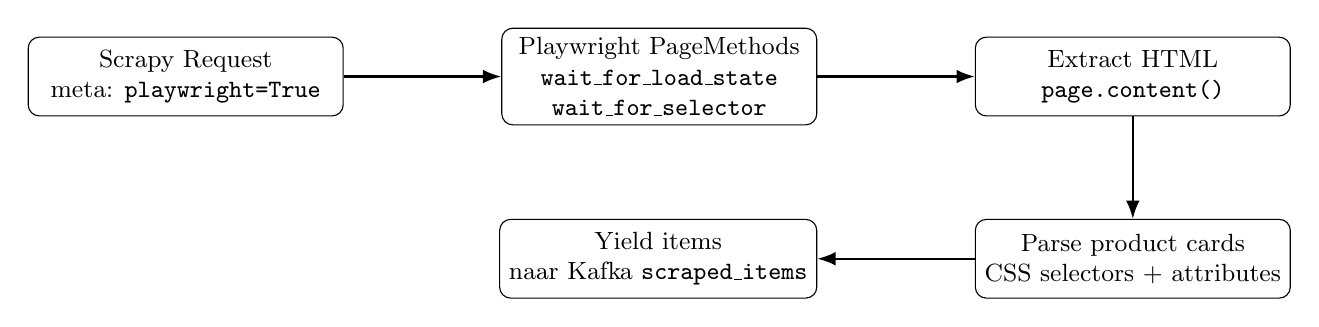
\begin{tikzpicture}[
        font=\small,
        node distance=1.3cm and 2.0cm,
        box/.style={draw, rounded corners, align=center, minimum width=4.0cm, minimum height=1.0cm},
        arrow/.style={-Latex, thick}
        ]
        \node[box] (req) {Scrapy Request\\meta: \texttt{playwright=True}};
        \node[box, right=of req] (pm) {Playwright PageMethods\\\texttt{wait\_for\_load\_state}\\\texttt{wait\_for\_selector}};
        \node[box, right=of pm] (html) {Extract HTML\\\texttt{page.content()}};
        \node[box, below=of html] (parse) {Parse product cards\\CSS selectors + attributes};
        \node[box, left=of parse] (yield) {Yield items\\naar Kafka \texttt{scraped\_items}};
        
        \draw[arrow] (req) -- (pm);
        \draw[arrow] (pm) -- (html);
        \draw[arrow] (html) -- (parse);
        \draw[arrow] (parse) -- (yield);
    \end{tikzpicture}
    \caption{Colruyt scraping flow met Scrapy-Playwright: requests renderen in een headless browser waarna HTML wordt uitgelezen en geparsed.}
    \label{fig:colruyt-flow}
\end{figure}

\subsection{Vergelijking van scraping-strategieën}

\begin{table}[H]
    \centering
    \renewcommand{\arraystretch}{1.25}
    \begin{tabular}{|p{3cm}|p{3.2cm}|p{3.2cm}|p{3.2cm}|}
        \hline
        \textbf{Kenmerk} & \textbf{Albert Heijn} & \textbf{Carrefour} & \textbf{Colruyt} \\
        \hline
        Databron & GraphQL API & Server-side HTML & Client-side JavaScript \\
        \hline
        Scraping-techniek & HTTP POST (JSON) & Scrapy HTML parsing & Scrapy + Playwright \\
        \hline
        Rendering nodig & Nee & Nee & Ja (headless browser) \\
        \hline
        Anti-bot complexiteit & Laag & Gemiddeld & Hoog \\
        \hline
        Stealthmaat\-regelen & Headers + impersonatie & Browser impersonatie & Multi-layer stealth + fingerprint spoofing \\
        \hline
        Paginatie & GraphQL response metadata & URL-parameter (\texttt{p}) & Query-parameter + JS-rendering \\
        \hline
        Performantie & Zeer hoog & Hoog & Lager \\
        \hline
        Foutgevoelig\-heid & Laag & Gemiddeld & Hoog (zonder mitigaties) \\
        \hline
        Onderhoud\-baarheid & Zeer goed & Goed & Complex \\
        \hline
        Gebruik Playwright & Nee & Nee & Ja \\
        \hline
    \end{tabular}
    \caption{Vergelijking van scraping-strategieën per supermarkt}
    \label{tab:scraper-comparison}
\end{table}

\subsubsection{Analyse en motivatie van de gekozen aanpak}

Tabel~\ref{tab:scraper-comparison} toont duidelijk aan dat voor elke supermarkt een verschillende scraping-strategie werd toegepast, afgestemd op de onderliggende technische architectuur van de website. Deze bron-specifieke benadering was noodzakelijk om zowel performantie als betrouwbaarheid te maximaliseren.

\paragraph{Albert Heijn}
Albert Heijn biedt productdata aan via een GraphQL-endpoint, wat directe en gestructureerde toegang tot prijs- en productinformatie mogelijk maakt. Hierdoor is geen HTML-parsing of JavaScript-rendering vereist. De scraper communiceert rechtstreeks met het backend-systeem via HTTP POST requests en ontvangt JSON-responses met een voorspelbare structuur.
Deze aanpak resulteert in een zeer hoge performantie en lage foutgevoeligheid, aangezien wijzigingen in de frontend geen impact hebben op de scraping-logica.

\paragraph{Carrefour}
Carrefour presenteert zijn zoekresultaten hoofdzakelijk als server-side gerenderde HTML-pagina’s. Hierdoor volstaat klassieke HTML-parsing met CSS-selectors. Omdat er geen complexe client-side rendering nodig is, kan scraping gebeuren zonder headless browser, wat de performantie ten goede komt.
Wel zijn beperkte anti-botmaatregelen aanwezig, waardoor browser-impersonatie werd ingezet om requests te laten lijken op regulier gebruikersverkeer.

\paragraph{Colruyt}
Colruyt vormt het meest complexe scraping-scenario. De website is sterk afhankelijk van client-side JavaScript, lazy-loading en interne API-calls, gecombineerd met actieve anti-botdetectie. Hierdoor is het gebruik van een headless browser (Playwright) noodzakelijk om de pagina correct te renderen voordat data geëxtraheerd kan worden.
Deze aanpak is intrinsiek trager en foutgevoeliger, maar onvermijdelijk om betrouwbare data te verkrijgen. Om dit te mitigeren werden geavanceerde stealthmaatregelen, aangepaste navigatiestrategieën en expliciet resourcebeheer geïmplementeerd.

\paragraph{Overkoepelende conclusie}
De vergelijking toont aan dat een uniforme scraping-oplossing onvoldoende zou zijn voor dit project. Door per databron de meest geschikte techniek te kiezen - GraphQL waar mogelijk, HTML-parsing waar voldoende, en headless rendering waar noodzakelijk - wordt een optimale balans bereikt tussen performantie, stabiliteit en onderhoudbaarheid.
Deze gelaagde aanpak onderstreept de flexibiliteit en schaalbaarheid van de gekozen scraping-architectuur.

\section{Opslag van ruwe data}

De spiders sturen hun resultaten niet rechtstreeks naar de databank, maar publiceren ruwe JSON-berichten naar het Kafka-topic \texttt{scraped\_items}. Kafka fungeert hierbij als buffer en ontkoppelingslaag tussen scraping en dataverwerking. Deze keuze biedt meerdere voordelen. Ten eerste kan data opnieuw verwerkt worden zonder opnieuw te scrapen. Ten tweede blijft de oorspronkelijke brondata beschikbaar voor validatie en foutanalyse. Verder maakt deze tussenlaag het systeem tolerant voor tijdelijke fouten en piekbelasting.

Deze stap sluit conceptueel aan bij event-gedreven architecturen waarbij data eerst als onbewerkte events wordt opgeslagen.

\section{Transformatielaag}

De normalizer consumeert berichten van het \texttt{scraped\_items}-topic en is verantwoordelijk voor:

\begin{itemize}
    \item productnamen opgeschoond;
    \item prijsnotaties genormaliseerd;
    \item eenheden geharmoniseerd;
    \item irrelevante HTML-elementen verwijderd.
\end{itemize}

Via \texttt{update\_or\_create} worden bestaande prijsrecords geüpdatet, wat voorkomt dat duplicaten ontstaan bij herhaalde scraping.
\begin{lstlisting}[language=Python, caption={Normalisatie en persistente opslag in \texttt{normalizer.py} (vereenvoudigd)}, label={lst:normalizer_upsert}]
def parse_decimal(value):
    try:
        return Decimal(str(value).replace(",", "."))
    except Exception:
        return None

shop, _ = Shop.objects.get_or_create(name=store_name)
product, _ = Product.objects.get_or_create(name=product_name)

ShopProduct.objects.update_or_create(
    product=product,
    shop=shop,
    defaults={
        "price_per_unit": price_per_unit,
        "barcode": barcode,
        "source_url": source_url,
        "scraped_at": scraped_at,
    },
)
\end{lstlisting}

Door transformatie los te koppelen van scraping wordt het systeem beter onderhoudbaar en uitbreidbaar. 

\section{Gestructureerde opslag}

Na normalisatie wordt de data opgeslagen in een PostgreSQL-databank via Django ORM. De databank bevat onder meer: Shop, Product, ShopProduct. Deze structuur laat toe om prijzen per winkel te vergelijken en historische updates bij te houden.

\section{Optimalisatie van productmatching}

In de initiële implementatie van de zoek- en winkelmandfunctionaliteit werd productmatching uitgevoerd via een eenvoudige substring-vergelijking op databankniveau, gebruikmakend van SQL \texttt{LIKE}-operatoren (of Django’s \texttt{icontains}-filter). Hoewel deze aanpak computationeel efficiënt is en een hoge recall oplevert, bleek de precisie onvoldoende voor betrouwbare prijsvergelijking.

Een typisch probleem hierbij is het zogenoemde \emph{substring collision}-effect. Zo resulteerde een zoekopdracht naar ``ijs'' (ice cream) ook in producten zoals ``rijst'', omdat de substring ``ijs'' voorkomt in het woord ``rijst''. Aangezien het systeem initieel de goedkoopste match selecteerde, leidde dit tot incorrecte resultaten waarbij irrelevante producten als beste optie werden voorgesteld. Dit had een negatieve impact op zowel de nauwkeurigheid van de vergelijking als de gebruikerservaring.


\subsection{Gelaagde similariteitsscore}

Om dit probleem te verhelpen werd een aangepaste matching- en rangschikkingslogica ontwikkeld op applicatieniveau. In plaats van een binaire match/no-match-benadering werd een meerlaags scoresysteem geïntroduceerd dat producten rangschikt op basis van hun linguïstische en semantische overeenkomst met de zoekterm.

De matchinglogica bestaat uit drie opeenvolgende lagen, waarbij elke laag een hogere tolerantiegraad heeft maar een lagere prioriteit krijgt in de rangschikking.

\subsubsection{Exacte overeenkomst (Laag 0)}

De hoogste prioriteit wordt toegekend aan een exacte, hoofdletterongevoelige overeenkomst tussen de productnaam en de zoekterm. Indien beide strings volledig overeenkomen, krijgt het product de laagst mogelijke score (\texttt{0.0}). Dit garandeert dat perfecte matches altijd bovenaan de resultaten verschijnen.

\subsubsection{Volledig-woordmatching via reguliere expressies (Laag 1)}

Indien geen exacte overeenkomst wordt gevonden, controleert het systeem of de zoekterm voorkomt als een afzonderlijk woord binnen de productnaam. Dit wordt gerealiseerd via reguliere expressies met woordgrenzen (\texttt{\textbackslash b}).

Deze aanpak vermijdt substringfouten en onderscheidt bijvoorbeeld correct ``ijs'' in ``vanille ijs'' van ``rijst'', waar ``ijs'' slechts deel uitmaakt van een groter woord. Bij meerdere geldige matches wordt een lichte voorkeur gegeven aan kortere productnamen, aangezien deze doorgaans generieker en relevanter zijn.

\subsubsection{Fuzzy matching met Levenshtein-afstand (Laag 2)}

Als laatste vangnet wordt fuzzy matching toegepast op basis van de Levenshtein-afstand. Dit algoritme berekent het minimale aantal karakterbewerkingen (invoegingen, verwijderingen of vervangingen) dat nodig is om de productnaam om te zetten in de zoekterm.

Om te garanderen dat fuzzy matches altijd lager gerangschikt worden dan exacte of volledig-woordmatches, wordt de afstand verhoogd met een vaste offset. Hierdoor blijven zelfs zeer goede fuzzy matches ondergeschikt aan semantisch sterkere overeenkomsten.


\subsection{Implementatie}

De matchinglogica werd geïmplementeerd binnen de Django-applicatielaag, aangezien dergelijke gelaagde ranking moeilijk efficiënt uit te drukken is in standaard SQL-query’s. Listing~\ref{lst:score_match} toont de kern van het scoringsmechanisme.

\begin{lstlisting}[language=Python, caption={Gelaagde productmatching met prioriteitsscores}, label={lst:score_match}]
def score_match(name: str, query: str) -> float:
    name, query = name.lower(), query.lower()

    # Laag 0: exacte match
    if name == query:
        return 0.0

    # Laag 1: volledig woord
    if re.search(rf"\b{re.escape(query)}\b", name):
        # lichte voorkeur voor kortere namen (meer generiek)
        return 1.0 + (len(name) - len(query)) / 100.0

    # Laag 2: fuzzy (Levenshtein)
    return float(levenshtein(name, query) + 2)
\end{lstlisting}


\subsection{Impact op systeemfunctionaliteiten}

De introductie van het scoresysteem had een directe impact op meerdere onderdelen van de applicatie:

\subsubsection{Herordening van zoekresultaten}
De zoekpagina haalt nu eerst een beperkte set kandidaatproducten op via \texttt{icontains}. Vervolgens wordt voor elk product een similariteitsscore berekend en worden de resultaten gesorteerd op \texttt{(score, prijs\_per\_eenheid)}. Hierdoor verschijnen de meest relevante producten bovenaan, zelfs indien zij niet de absoluut laagste prijs hebben.

\subsubsection{Slimme winkelmandberekening}
Bij het automatisch samenstellen van een goedkoopste winkelmand wordt niet langer blind het goedkoopste product geselecteerd. In plaats daarvan wordt eerst bepaald welke producten tot de beste matchcategorie behoren. Indien enkel lage-kwaliteit fuzzy matches beschikbaar zijn, wordt dit beschouwd als een lage betrouwbaarheidssituatie en wordt automatisch een nieuwe, gerichte scraping-opdracht ingepland.


\subsection{Conclusie}

Door over te stappen van een eenvoudige substringvergelijking naar een gelaagde similariteitsscore werd het aantal foutieve productmatches aanzienlijk verminderd. De combinatie van volledig-woorddetectie en Levenshtein-afstand biedt een evenwicht tussen strikte nauwkeurigheid en flexibiliteit voor variabele productbenamingen. Deze aanpak verhoogt zowel de betrouwbaarheid van prijsvergelijkingen als de kwaliteit van de gebruikerservaring.


\section{Geplande updates}

Naast gebruikersgestuurde scraping wordt ook proactieve data-verversing voorzien via \texttt{scheduler.py}. Dit script publiceert op vaste tijdstippen (dagelijks om 02:00) scraping-opdrachten voor een set basisproducten.

Hierdoor bevat het systeem steeds recente data, zelfs zonder actieve gebruikers.
\begin{lstlisting}[language=Python, caption={Nightly refresh jobs publiceren in \texttt{scheduler.py} (vereenvoudigd)}, label={lst:scheduler_nightly}]
def publish_job(query: str, reason: str):
    payload = {
        "query": query,
        "reason": reason,
        "requested_at": datetime.now(timezone.utc).isoformat(),
    }
    producer.send(TOPIC, key=query.encode("utf-8"), value=payload)

def nightly():
    for term in SEARCH_TERMS:
        publish_job(term, reason="nightly")
    producer.flush()

schedule.every().day.at("02:00").do(nightly)
\end{lstlisting}



\section{Docker}


Alle componenten van het systeem draaien als afzonderlijke Docker-containers:

\begin{itemize}
    \item Django webapplicatie
    \item PostgreSQL databank
    \item Kafka broker
    \item Scraper worker
    \item Normalizer
    \item Scheduler
\end{itemize}

Via \texttt{docker-compose} worden deze containers samen opgestart en via een gedeeld netwerk met elkaar verbonden.
\begin{lstlisting}[language=YAML, caption={Uittreksel \texttt{docker-compose.yaml}: services en Kafka listeners}, label={lst:docker_compose}]
broker:
  image: confluentinc/cp-kafka:7.6.1
  ports:
    - "9092:9092"     # host access
    - "29092:29092"   # container network
  environment:
    KAFKA_LISTENERS: PLAINTEXT_INTERNAL://0.0.0.0:29092,PLAINTEXT_HOST://0.0.0.0:9092
    KAFKA_ADVERTISED_LISTENERS: PLAINTEXT_INTERNAL://broker:29092,PLAINTEXT_HOST://localhost:9092

web:
  build: .
  depends_on: [db, broker]
  ports: ["8000:8000"]

scraper-worker:
  build: .
  depends_on: [db, broker]
  command: ["python", "scripts/scraper_worker.py"]
\end{lstlisting}
 Omgevingsvariabelen (zoals databank- en Kafka-configuratie) worden centraal beheerd via een \texttt{.env}-bestand.

Deze aanpak garandeert reproduceerbaarheid, vereenvoudigt deployment en maakt horizontale schaalvergroting mogelijk door meerdere workers te starten.

\section{Conclusie}

Het prototype combineert een gebruiksvriendelijke interface met een modulaire en schaalbare backend-architectuur. Door de scheiding tussen scraping, opslag en transformatie sluit het ontwerp nauw aan bij zowel academische literatuur als hedendaagse best practices.

Deze architectuur biedt een solide basis voor verdere uitbreidingen, zoals automatische planning van scrapingtaken, ondersteuning voor bijkomende websites en grootschalige data-analyse.







%The prototype starts at outlining the work. This is meant to be used by an average student without extra knowlage of programming and access to the internet. That points to a need of simple ui interface and the rest needs to happen behind the sines of it.
%
%The choice of the languages and frameworks is wide. Based on the articles \autocitate{5BestLang, StateofArt, BestPractice2025, PvsJS} Python was chosen for the main language of scraping. This choice was dectated by the amount of libraries thst are avilable, available knowlage of co-promoter and the ease of use for the web-scraping beginners. As well as an outlook for large data processing in the future.
%
%The structure of web scraping is outlined in the  \autocitate{Laender2002} with inspiration for Kafka usage from \autocitate{Eyzenakh2021} and \autocitate{Kafka2015} with its diagram.
%
%Verder in de bespreking met de co-promoter zijn we gekomen tot de volgende architectuur:
%
%
%Architectuur uitwerken: in bespreking met co-promoter heeft hij state of art uitgelegd en daarbij volgende architectuur van de app was voorgesteld:
%*pic*
%*Bechrijving daarvan*
%
%Geprobeerd beautiful soup + requests, daar wordt er makkelijk gedetecteerd dat het geen echte persoon is.
%Daar 403 en 456 tegengekomen. En ik werd geblocked door cloudfaire van carrefour met gewone requests.
%
%Daarna van Co-promoter aangeraden om scrapy te gebruiken en beter scrapy impersenate om headers van de browser na te doen. Aanpak: 1. Graphql van AH aanspreken met json als een antwoord. 2. Carrefour de pagina zelf scrapen. 3. Coloryt scrapen van de pagina met playwrite om js elementen te loaden.
%
%
%https://github.com/JaapWestera/albert-heijn-graphql-api/tree/main?tab=readme-ov-file
%
%https://www.scrapingbee.com/blog/scrapy-playwright-tutorial/
%https://medium.com/@geneng/web-crawling-made-easy-with-scrapy-and-rest-api-ed993e84abd3